\documentclass{article}

% packages for UCR big table
\usepackage{booktabs}
\usepackage{array}
\usepackage{datatool}
\usepackage{longtable}

% file including commands for drawing our long tables
% code from: https://tex.stackexchange.com/questions/447202/highlight-maximum-values-for-each-row-in-large-csv

% commad for drawing ucr table
% \newcommand{\drawucrepochs}{
% \drawtable{"results/Experiments_my_own - UCR_all_important_columns.csv"}{1}{Test accuracy scores for all 128 UCR datasets, run with a fixed number of epochs instead of a fixed number of optimization steps.}{tab:ucr_all}{UCR_DATA}
% }

%\newcommand{\drawucrepochs}{
%\drawtable{"results/Experiments_my_own_UCR_all_important_columns_alpha_3.csv"}{1}{Test accuracy scores for all 128 UCR datasets, run with a fixed number of epochs instead of a fixed number of optimization steps.}{tab:ucr_all}{UCR_DATA}
%}

\newcommand{\drawucrsteps}{
% "results/UCR_results_steps_important_columns.csv"
\drawtable{"../openreview/finalized_results/Finalized UCR experiments - ADL project - [For report] features_UCR_steps_noise_complete.csv"}{1}{Test accuracy scores for all 128 UCR datasets.}{tab:ucr_all_steps}{UCR_DATA_steps}
}

\newcommand{\drawueasteps}{
% results/UEA_results_steps_important_columns.csv
\drawtable{"../openreview/finalized_results/Finalized UEA experiments - ADL project - [For report] features_UEA_steps_noise_complete.csv"}{1}{Test accuracy for all the datasets in the UEA archive.}{tab:uea_all_steps}{UEA_DATA_steps}
}

%\newcommand{\drawueaepochs}{
%\drawtable{"results/Experiments_my_own - UEA_important columns (latex).csv"}{1}{Test accuracy for all the datasets in the UEA archive, run with a fixed number of epochs instead of a fixed number of optimization steps.}{tab:uea_all_epochs}{UEA_DATA_epochs}
%}

%\newcommand{\tableone}{
%\drawtable{"results/Experiments_my_own - Table 1.csv"}{1}{Scores for all the methods on a selection of the UCR datasets. Missing scores are indicated by '-'.}{tab:table1}{T1DATA}
%}

\newcommand{\drawtable}[5]{
% arg 1: csv file name in the results folder
% arg 2: column number to exclude: columns before that are not considered for the max() operation
% arg 3: caption of the table
% arg 4: label of the table
% arg 5: name of the database created and used by the datatools package. Choose a unique name for this.


% "results/Experiments_my_own - UCR_all_important_columns.csv"
% \DTLdisplaylongdb[caption={Full accuracy results on all 128 UCR datasets}, label={tab:ucr_all}]{DATA}

\DTLloadrawdb[]{#5}{#1}
\DTLforeach{#5}{}{                                % iterate over rows
    \def\theMax{0}                                  % set max to zero
    \DTLforeachkeyinrow{\thisValue}{                % iterate over cols
        \ifthenelse{\dtlcol>#2}{                     % ignore columns before that
            \DTLmax{\theMax}{\theMax}{\thisValue}   % compare max with current value
        }{}
    }       
    % Now \theMax should be maximal

    \DTLforeachkeyinrow{\thisValue}{                % iterate again over cols
        \ifthenelse{\dtlcol>#2}{                     % ignore columns before that
            % If current Value is maximal, make it bold
            \ifthenelse{\DTLisieq{\thisValue}{\theMax}}{
                \DTLreplaceentryforrow{\dtlkey}{\textbf{\theMax}}
            }{}
        }{}
    }           
}
% left alight string and int values in the table
\renewcommand{\dtlstringalign}{l}
\renewcommand{\dtlrealalign}{l}

\renewcommand{\dtldisplaystarttab}{\hline} % horizontal line before header
\renewcommand{\dtldisplayafterhead}{\hline} % horizontal line after header
\DTLdisplaylongdb[caption={#3}, label={#4}]{#5}
}

\usepackage{color, soul}
% if you need to pass options to natbib, use, e.g.:
%     \PassOptionsToPackage{numbers, compress}{natbib}
% before loading neurips_2019

% ready for submission
% \usepackage{neurips_2019}

% to compile a preprint version, e.g., for submission to arXiv, add add the
% [preprint] option:
%     \usepackage[preprint]{neurips_2019}

% to compile a camera-ready version, add the [final] option, e.g.:
     \usepackage[final]{neurips_2019}

% to avoid loading the natbib package, add option nonatbib:
%     \usepackage[nonatbib]{neurips_2019}

\usepackage[utf8]{inputenc} % allow utf-8 input
\usepackage[T1]{fontenc}    % use 8-bit T1 fonts
\usepackage{hyperref}       % hyperlinks
\usepackage{url}            % simple URL typesetting
\usepackage{amsfonts}       % blackboard math symbols
\usepackage{nicefrac}       % compact symbols for 1/2, etc.
\usepackage{microtype}      % microtypography
\usepackage{tcolorbox}      % boxed text with notes to teacher of ADL course
\usepackage{arydshln}       % dashed line in table

% References added by Felix (not part of NeurIPS template)
\usepackage{natbib}
\bibliographystyle{abbrvnat}
\setcitestyle{authoryear,open={(},close={)}}

\title{[Re] Unsupervised Scalable Representation Learning for Multivariate Time Series}

% The \author macro works with any number of authors. There are two commands
% used to separate the names and addresses of multiple authors: \And and \AND.
%
% Using \And between authors leaves it to LaTeX to determine where to break the
% lines. Using \AND forces a line break at that point. So, if LaTeX puts 3 of 4
% authors names on the first line, and the last on the second line, try using
% \AND instead of \And before the third author name.


\author{%
  Felix Liljefors* \\
  KTH Royal Institute of Technology \\
  \texttt{felixlil@kth.se} \\
  \And
  Moein Sorkhei* \\
  KTH Royal Institute of Technology \\
  \texttt{sorkhei@kth.se} \\
  \AND
  Sofia Broomé* \\
  KTH Royal Institute of Technology \\
  \texttt{sbroome@kth.se}
}



\begin{document}

\maketitle
%*****************INTRODUCTION****************************************************

% \begin{abstract}
%     We have reimplemented the paper \textit{Unsupervised Scalable Representation Learning for Multivariate Time Series} by FranceschiUnsupervised2019, as part of the Replications track of the NeurIPS Reproducibility Challenge 2019.
% \end{abstract}

\section{Introduction}

The paper \textit{Unsupervised Scalable Representation Learning for Multivariate Time Series} by \cite{FranceschiUnsupervised2019} presents an unsupervised approach to learning representations for time series that can be used for subsequent classification. An encoder architecture with dilated causal convolutional blocks is trained to minimize a triplet loss. The triplet loss is based on the idea that a subseries, $x_{pos}$, of a time series, $x_{ref}$, should be closer to $x_{ref}$ in representation space than the representation of a randomly sampled time series from the dataset, $x_{neg}$. This type of loss was first introduced by \cite{ogtriplet}.

To evaluate the strength of the learned representations, an SVM classifier is trained using the labels corresponding to these representations. The evaluation is performed on 159 datasets, together constituting the main benchmarking datasets for time series. The first group of datasets (the UCR Archive, \cite{UCRArchive2018}) contains univariate, short (between 15 and 2844 time steps) series; the second group, the UEA dataset (\cite{bagnall2018uea}), contains multivariate time series of up to 1345 dimensions and varying sample lengths. The last dataset, the Individual Household Electric Power Consumption (IHEPC) dataset from the UCI Machine Learning Repository (\cite{Dua:2019}), is a single seven-dimensional time series with more than two million time steps. The authors' intention with using this variety of datasets is to show the universality of their method, which is one of their main claims.

We have re-implemented the authors' method from scratch as best as we could by using only the paper as instruction. It should be noted that a code repository for the article was made public by the authors, but this was not employed for the purpose of investigating the replicability of the work starting from scratch. This means that we adhere to the Replication track of the Reproducibility challenge for NeurIPS 2019. Our implementation, as well as the authors', was made using the Pytorch (\cite{Pytorchpaszke2017automatic}) library and can be found at \url{https://github.com/lilfelix/reproducibility_NeurIPS19}.

The main motivation to do a full replication study, avoiding the use of readily provided code, is to better be able to detect if there are parts of the implementation that are crucial for the results, but not presented as such in the original paper. This risk exists generally in machine learning (\cite{LiptonTroubling}), and has in particular been brought to light for deep learning (e.g. \cite{henderson2017reinforcement}, \cite{Hyper1Melis}), due to the latter's typically vast number of hyperparameters to tune.

%\begin{tcolorbox}[arc=0mm]{
%In the report these boxes contain notes specifically addressed to the teacher of DD2412.
%These boxes will be removed before our submission to the NeurIPS19 Reproducibility challenge.
%\end{tcolorbox}

\subsection{Target questions}

In this report, we mainly address the following questions.

\begin{itemize}
    \item Can the classification and regression results be reproduced using only the article's description of the method?
    \item Can we reproduce the claimed transferability of the method and its proposed success on sparsely labeled datasets?
    \item Which missing instructions for the experiments might, if relevant, have affected the results?
    \item Which 'hidden' assumptions, that mattered for the results, were made by the authors?
    
    %Can we observe the main advantages of the authors' method concerning transferability and success in sparsely labeled datasets?
\end{itemize}

\subsection{Additional contributions}
We present results for the authors' method on three additional datasets from the UCR Archive: DodgerLoopDay, DodgerLoopGame and DodgerLoopWekend. These results can be found in Table 6 of the supplementary material.

The rest of the article is organized as follows: Section \ref{expmet} presents the implementation details and the results, in Section \ref{sect:disc} we discuss the findings, and Section \ref{conc} is dedicated to the conclusions.

%*****************BACKGROUND******************************************************
% \section{Background}
% Put any background paragraphs here that can be useful for the reader of this report, without re-writing the original paper.
% 
% \subsection{Unsupervised training and encoder architecture}
% Describe in short the triplet loss, samples, and the encoder architecture with dialated convolutions.


%*****************REPRODUCIBILITY*************************************************
\section{Experimental methodology and implementation details}
\label{expmet}
In Sections \ref{ucr}-\ref{ihepc}, we will group the reproducibility experiments into the three dataset groups (UCR, UEA and IHEPC). First, we will describe our general experimental methodology for this study and some assumptions not mentioned in the original article that were necessary to make for all three groups of datasets. A strength of the original paper is that experimental hyperparameters are listed to a greater detail than is typically done in deep learning papers. Nevertheless, there are a number of design choices of importance for the implementation that were not mentioned in the article. 

We implemented \textbf{Algorithm 1} from the paper (described in pseudo-code), to sample three subseries\footnote{A subseries here is a contiguous sub-sequence of a time series.} $x_{ref}, x_{pos}$ and $x_{neg}$, used to compute the triplet loss. This algorithm is described by the authors as generally applicable to all datasets. However, they also mention a variation of \textbf{Algorithm 1}, which they claim speeds up the training time for datasets with fixed length time series, yet produces no noticeable difference in the computed loss. We did not implement this variation for fixed length time series, but instead used \textbf{Algorithm 1} for all experiments. In the case of multivariate datasets, we assume that the length of a subseries, e.g. size($x_{ref}$), is the same across all dimensions of the time series being sampled from. In other words, when sampling $x_{ref}$ from some $d$-dimensional time series $y$, size($x^{i}_{ref}$) is the same for all $i\in[1,d]$.

Notably, except for IHEPC, the authors state that they have used a batch size of 10 throughout their experiments. Mini-batch training requires sequence padding when there are samples of different lengths. This is the case for these experiments since subseries are explicitly sampled at different lengths from the dataset (see Algorithm 1 in \cite{FranceschiUnsupervised2019}). However, there is no mention of how this padding is carried out in the article. For our experiments, we zero-pad the samples to the maximal sample length for each batch.

%%%%%%%%%%%%
% (I don't think the below belongs here. The varying length padding doesn't matter since we don't sample from it anyway. And the normalization is already mentioned in the article:)
%Additionally, a portion of the UCR as well as UEA datasets have varying length samples. We zero-pad these samples before sampling and batching (ensuring not to sample from the zero-padding). For the datasets that weren't already standardized, we ensured they had zero-mean and unit variance, as described in the paper. For the multivariate datasets this entaild standardizing each feature separately.
%%%%%%%%%%%



Another training detail not made explicit in the article is whether the representations used for classification should be obtained from full samples of the datasets (i.e. of length $T$, if $T$ is the number of time steps for one sample), or rather from randomly sampled subseries of the samples (i.e. of length $T'$, where $T' \in [1,T]$). For our experiments, we used the full samples (length $T$) in order to use the training set maximally when training the classifier.

Regarding the SVM training, a hyperparameter optimization is performed for the weighting $C$ of the error term using cross-validation across the training set. The authors indicate that they avoided this cross-validation for datasets with a small number of training samples or datasets with few training samples per class. In lack of an exact list of which datasets they refer to, we avoided the hyperparameter search only for the datasets that fell below the size limit set by the cross-validation tool of scikit-learn (\cite{scikit-learn}).

%Regarding the SVM training, there is a paragraph in the appendix of the article stating that for datasets where the number of training samples was 'too small', a penalty $C= \infty$ (no regularization) was used. Since we could not know what constitutes a too small training set, and since SVM training did not take very long, we set out to include $C= \infty$ in the grid search for $C$ for all datasets. When starting to run, we however quickly discovered that scikit-learn shows a warning when a dataset has fewer than five samples per class. We suspect that these are the datasets that were deemed too small by the paper authors. Therefore, in the end, we avoided the grid search and only trained with $C= \infty$ for these datasets. Furthermore, there are hyperparameters for the choice of SVM in scikit-learn (\cite{scikit-learn}) which are not specified in the paper. For our experiments, we settled for the default scikit-learn hyperparameters. We used five folds for the SVM cross-validation.

% \begin{tcolorbox}
% Lastly, it is specified in the article's appendix that the models were trained for 2000 optimization steps when $K \ge 10$ and 1500 steps otherwise. At the same time, they give an example saying that these number of steps corresponded to 20 epochs for a dataset of size 1000. Unfortunately, this confused us and we instead trained all datasets for 20 epochs when $K \ge 10$ and 15 epochs otherwise. This has led to the following consequences for the current report: all models with less than 1000 samples have been trained with fewer steps than in the article, and all models with more than 1000 samples have been trained with more steps than in the article. \textit{We will update these numbers before Nov 6th. For computational reasons, it was not feasible to rerun our results for all 159 datasets before Nov 1st. We suspect that the results will be quite similar, since the loss flattened out very quickly for most datasets.}
% \end{tcolorbox} 

%*****************UCR*************************************************************
\newpage
\subsection{The UCR Time Series Classification}
\label{ucr}

The UCR Archive contains 128 univariate datasets. Each dataset consists of training and test time series which may have different lengths and missing values. The paper's authors decided to not use the three datasets with missing values (DodgerLoopDay, DodgerLoopGame and DodgerLoopWekend). However, the UCR Archive contains modified versions of these datasets with linearly interpolated values that we used. Our motivation for this is that the UCR Archive briefing document recommends that all available datasets are used, to allow for comprehensive comparisons and avoid cherry-picking results.

%I removed the below because it's not really relevant to why we pad.
%The archive also contains 11 datasets with varying length samples which we zero-padded to the length of the longest sample per mini-batch, before subsampling. The subsamples fed to the encoder are then zero-padded again to the longest subsampled length of the batch.

For the task of time series classification on the UCR Archive datasets, the authors consider other state-of-the art methods, some of which are based on neural networks. More specifically, they compare their method to neural network methods, both unsupervised (TimeNet, \cite{TimenetMalhotraTVAS17}; RWS, \cite{RWSwu2018random}) and supervised (ResNet, \cite{ResNetHe2015}), and non-neural network methods, both unsupervised (Dynamic Time Warping (DTW)) and supervised (HIVE-COTE, \cite{hivecote}; ST, \cite{STBostrombagnall}; BOSS, \cite{BOSSSchafer:2015:BCT:2833463.2833468}; EE, \cite{EELines2015}).
%They also compare their results with DTW (one-nearest neighbor classifier) and ResNet
%(\hl{cite authors of methods})
The use of ResNet as a baseline in the paper is motivated by referencing an extensive review made by \cite{fawaz2019deep}, who found it to be the best supervised neural network method for time series classification.
%(\hl{cite Ismail}).


In Table 1 of the paper, the authors present their accuracy scores on 6 datasets from the UCR Archive, together with baseline\footnote{The authors adapted the results from \url{http://www.timeseriesclassification.com/singleTrainTest.csv}, \url{https://www.cs.ucr.edu/~eamonn/time_series_data_2018/}, and \url{https://github.com/hfawaz/dl-4-tsc/blob/master/results/results-uea.csv}}
accuracy scores from non-neural network models (both supervised and unsupervised). In a similar fashion, Table \ref{tab:table1non} in this report presents our replicated accuracy scores for the same datasets, together with the original results from the paper for comparison. We also introduce a comparison of our replicated scores and the authors' against neural network models in Table \ref{tab:table1nn}.

%To provide quick overview of the the results,
Table \ref{tab:table1non} and \ref{tab:table1nn} present the highest accuracy  for each dataset, across all values of $K \in \{1,2,5,10\}$. Results for all values of $K$ and all datasets can be found in Table 6 of the supplementary material.
Further, these tables contain accuracy scores for three additional UCR datasets (not presented in the original paper's Table 1), for which we also have baseline scores of \textit{both} RWS and TimeNet (see Table \ref{tab:table1nn}). These are presented below the dashed line, and provide a comparison between the non-neural network scores in Table \ref{tab:table1non} and the neural network scores in Table \ref{tab:table1nn}.

%Table \ref{tab:table1non} shows the highest test accuracy we achieved among different values of $K$ compared the best performance that the authors achieved along with other non-neural-network methods. Table \ref{tab:table1nn} shows the best performance compared with neural network methods. We observe that there are very few datasets for which we have the scores of both TimeNet and RWS. Hence the comparison is incomplete. Note that for the other methods, we are just reporting the numbers mentioned in the paper \footnote{The authors adapted the results from \url{http://www.timeseriesclassification.com/singleTrainTest.csv}, \url{https://www.cs.ucr.edu/~eamonn/time_series_data_2018/}, and \url{https://github.com/hfawaz/dl-4-tsc/blob/master/results/results-uea.csv}}.

\begin{table}[h!]
%\setlength{\tabcolsep}{7.5pt}
\caption{Our best achieved scores compared to the authors' best achieved scores along with the scores for all the non-neural-network methods for some UCR datasets.}
\label{tab:table1non}
\centering
\begin{tabular}{llllllll}
    \hline
                        &                &                & \vrule    &            &    Baseline        &          &  \\

    Dataset             & Ours           & Authors'       & \vrule   DTW        & ST         & BOSS       & HIVE-COTE      & EE         \\
    \hline
    ECGFiveDays         & \textbf{1}          & \textbf{1}     & \textbf{1}      & 0.984      & \textbf{1} & \textbf{1}     & 0.82       \\
    DiatomSizeReduction & 0.987 & \textbf{0.993} & 0.967      & 0.925      & 0.931      & 0.941          & 0.944      \\
    FordB               & 0.785          & 0.81           & 0.62       & 0.807      & 0.711      & \textbf{0.823} & 0.662      \\
    Ham                 & \textbf{0.762} & 0.724          & 0.467      & 0.686      & 0.667      & 0.667          & 0.571      \\
    Phoneme             & 0.225           & 0.289          & 0.228      & 0.321      & 0.265      & \textbf{0.382} & 0.305      \\
    SwedishLeaf         & 0.922          & 0.931          & 0.792      & 0.928      & 0.922      & \textbf{0.954} & 0.915      \\ \hdashline
    ECG5000             & 0.928          & 0.94          & 0.924      & 0.944      & 0.941      & \textbf{0.946} & 0.939      \\
    TwoPatterns         & \textbf{1}     & \textbf{1}     & \textbf{1} & 0.955      & 0.993      & \textbf{1}     & \textbf{1} \\
    Wafer               & 0.998          & 0.995          & 0.98       & \textbf{1} & 0.995      & 0.999          & 0.997      
    \end{tabular}
\end{table}

%\renewcommand{\arraystretch}{2}
\begin{table}[h!]
\setlength{\tabcolsep}{7.5pt}
\caption{Our best achieved scores compared to the authors' best achieved scores along with the scores for supervised and unsupervised neural network methods for some UCR datasets. Missing scores are indicated by '-'.}
\label{tab:table1nn}
\centering
\begin{tabular}{llllll}
\hline
                    &                &                &\vrule & Baseline \\

Dataset             & Ours           & Authors'       &\vrule ResNet         & TimeNet & RWS   \\
\hline
ECGFiveDays         & \textbf{1}          & \textbf{1}     & 0.99           & -       & -     \\
DiatomSizeReduction & 0.987 & \textbf{0.993} & 0.301          & -       & -     \\
FordB               & 0.785          & \textbf{0.81}  & -              & -       & -     \\
Ham                 & 0.762          & 0.724          & \textbf{0.8}   & -       & -     \\
Phoneme             & 0.225           & 0.289          & \textbf{0.333} & -       & -     \\
SwedishLeaf         & 0.922          & 0.931          & \textbf{0.955} & 0.901   & -    \\ \hdashline
ECG5000             & 0.928          & \textbf{0.94} & 0.935          & 0.934   & 0.933 \\
TwoPatterns         & \textbf{1}     & \textbf{1}     & \textbf{1}     & 0.999   & 0.999 \\
Wafer               & \textbf{0.998}          & 0.995 & \textbf{0.998} & 0.994   & 0.993  

\end{tabular}
\end{table}
\newpage
\subsection{Sparse labeling experiment}

Figure \ref{fig:sparse} shows our reproduction of the sparse labeling experiment of Section 5.1.1 of the paper, where a comparison is made between the authors' method and ResNet when training on fractions of the labeled data from a randomly chosen dataset (TwoPatterns). Just as in the original article, there is a striking difference between the ResNet and the encoder model from the article on the smaller portions ($<50\%$) of training data. Hence our results are in line with the authors' claim; an SVM trained on labeled representations from their architecture performs better than ResNet trained on the raw data when training data is sparsely labeled.

% that an SVM trained on labeled encoded representations from their architecture
% %of a randomly chosen labeled set (TwoPatterns in this case)
% outperforms the supervised neural network ResNet trained on a labeled set of the same size, when the amount of labeled data is reduced for both models.
% %This is especially noticable when the percentage of labeled data is small.

The shapes of the ResNet graphs (in blue and red in Figure \ref{fig:sparse}) are different. %between the two plots in Figure \ref{fig:sparse}
This is likely explained by
%the fact that we do not know which type of ResNet architecture and hyperparameters that the authors used
%Furthermore, crucial information is missing regarding the sparse labeling experiment (Section 5.1.1 in the article).
%In this experiment, SVM classification on the learned representations is compared to fully supervised classification using ResNet (\cite{ResNetHe2015}) across different amounts of labeled data on one of the UCR datasets (TwoPatterns).
%Surprisingly,
the fact that, surprisingly, there are no details about which ResNet architecture was used for this experiment, or with which set of hyperparameters, or whether it had been pre-trained in any capacity. It is possible that this is made clear in the public code repository. Yet, for the sake of the replications track, we did not look this up.

Instead, for this experiment, we chose to train the least deep among the standard ResNets provided by PyTorch: ResNet-18. This choice was made considering the low dimensionality of the time series data compared to image data which ResNet is typically trained on. Specifically, this experiment was only run on univariate data from the UCR dataset, which further motivated our choice of an as-simple-as-possible ResNet architecture. We trained the network from scratch since it required modified input dimensions compared to the standard ResNet from the Pytorch library.

\begin{figure}[h!]%
    \centering
    \subfloat{{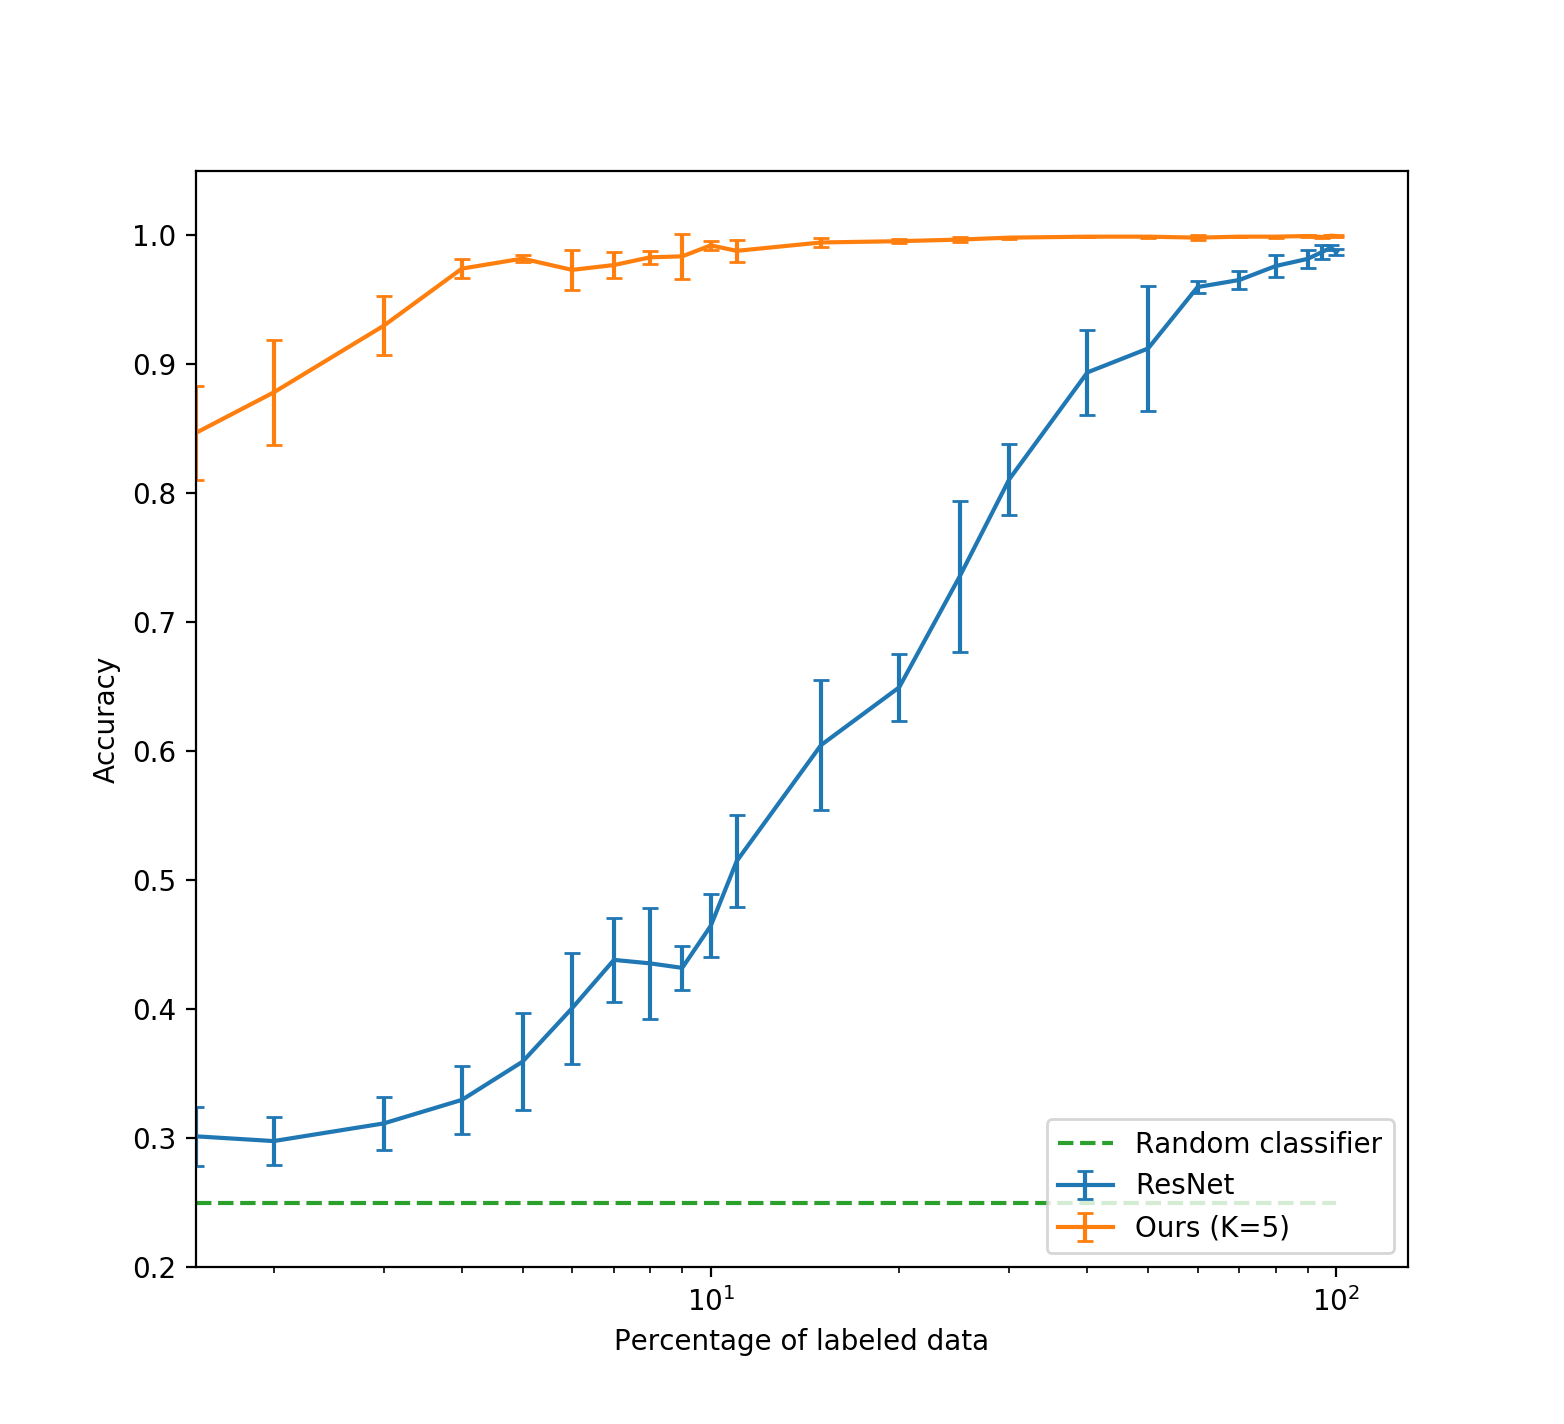
\includegraphics[width=6.8cm]{figures/fig.png} }}%
    \qquad
    \subfloat{{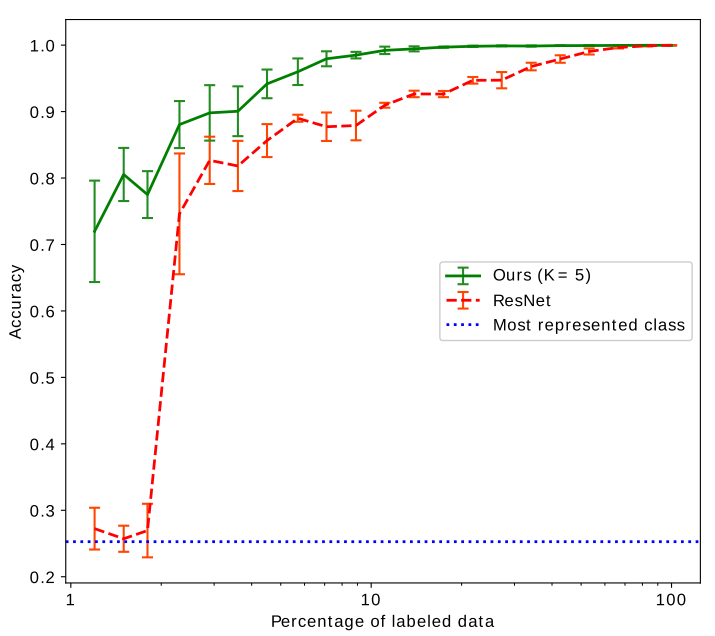
\includegraphics[width=6.3cm]{figures/sparse.png} }}%
    \caption{Reproduction of Figure 4 from the original article (right). The same striking difference between ResNet and the authors' method is observed when training on a limited amount of labeled data.}%
    \label{fig:sparse}%
\end{figure}

\subsection{Transferability experiment}
In the supplementary material, we reproduced the transferability experiment from the original article. These results are shown in Table 6 of the supplementary material, in the column entitled FordA. The idea for the transferability was to train an encoder on the FordA dataset, then pass samples from the other datasets through this encoder and see how well the SVM can learn from training on those representations with labels. The idea with the experiment was to show the generality of such a learned encoder and to show that classification results are comparable even if the encoder is trained on one dataset and produces representations on other datasets. Our results are very similar to the authors' results in Table S1 of the article.

%*****************UEA*************************************************************
\subsection{The UEA Time Series Classification}
\label{uea}

The UEA archive contains 30 multivariate datasets, with the dimensions per sample ranging from 2 to 1345. Some of these datasets have missing values. While the handling of missing values was not described in the paper, we chose to linearly interpolate these values before training the encoder. For the four datasets with the longest samples (EigenWorms, EthanolConcentration, MotorImagery and StandWalkJump) we needed to adjust the batch size to below 10 in order to fit the GPU memory. These adjustments can be seen in Table \ref{tab:batch}.

\begin{table}[h!]
\caption{Adjusted batch sizes for datasets with the longest sample lengths}
\label{tab:batch}
\begin{tabular}{lllll}
\hline
Dataset & EigenWorms & EthanolConcentration & MotorImagery & StandWalkJump \\
\hline
$K=5$     & 4          & 10                   & 6            & 8             \\
$K=10$    & 2          & 10                   & 6            & 8             \\
$K=20$    & 1          & 8                    & 6            & 8 \\       \hline    
\end{tabular}
\end{table}

% \begin{tcolorbox}[colback=white]
% A few of the UEA datasets (MotorImagery, StandWalkJump, SpokenArabicDigits and EigenWorms) contained very long samples which could not fit on a single GPU with a batch size of ten, as was done in the article. However, the Nvidia Titan XP used in the article has 1Gb more memory than the one we ran on. Since we are in any case re-running all experiments with the correct number of training steps for Nov 6th, we will run the largest datasets on an Nvidia Titan XP before that as well, to see if a batch size ten fits on that one. For this reason, we aim to complete the report with these results by Nov 6th.
% \end{tcolorbox}

The authors compare their scores on the UEA datasets to that of $\mathrm{DTW_D}$. $\text{DTW}_D$, an extension of DTW, is the best baseline known in the multivariate setting, according to the paper. In Table \ref{tab:uea}, we present our best achieved accuracy (taken among results using different values of $K$) next to the authors' scores, along with the scores of $\mathrm{DTW_D}$ for a random selection of UEA datasets.
%Similarly to the UCR case, for the we are only reporting the numbers from the paper for $\mathrm{DTW_D}$.

As can be seen, our best scores closely match the best scores of the authors for these datasets. Our full scores on all the UEA datasets except InsectWingBeat can be found in Table 7 of the supplementary material. InsectWingBeat with its large number of training samples was unfeasible for our time horizon to train the SVM with when using scikit-learn, see the discussion in Section \ref{sect:disc}. For $K=10$, the training would have taken more than 12 hours, so we decided to not include this dataset.


\begin{table}[h!]
\caption{Best scores achieved in our experiments compared to the authors' best scores along with the $\mathrm{DTW_D}$ method on some UEA datasets}
\label{tab:uea}
\centering
\begin{tabular}{llll}
    \hline
               &       &          & \vrule Baseline \\
    
    Dataset          & Ours  & Authors' &\vrule $\mathrm{DTW_D}$  \\
    \hline
    ArticularyWordRecognition & 0.983           & \textbf{0.987}    & \textbf{0.987} \\
    AtrialFibrillation        & \textbf{0.333}   & 0.2      & 0.2   \\
    Libras                    & \textbf{0.889} & 0.883             & 0.87           \\
    NATOPS                    & 0.922 & \textbf{0.944}    & 0.883          \\
    UWaveGestureLibrary       & \textbf{0.903}          & 0.884             & \textbf{0.903}
\end{tabular}
\end{table}


%*****************IHEPC***********************************************************
\subsection{The IHEPC experiment}
\label{ihepc}
The Individual Household Electric Power Consumption (IHEPC) is a seven-dimensional time series (not including the temporal dimension) containing over two million measurements. These measurements were split by the authors into train and test sets of 500,000 and $\sim$1,500,000 values, respectively. The paper does not mention the multivariate property of the IHEPC dataset and describes that the data was normalized in the same way as the univariate UCR datasets (multivariate normalization is described separately). Further, the plotted result for the IHEPC experiment (Figure 5 in the paper) shows only one feature (active power consumption), leading us to believe that only this feature was used. This belief was also strengthened when we trained the encoder on a single time series of length 500,000 measurements, since using all seven features simply requires more GPU memory than the authors specified in the report (16 GB). Lastly, the dataset has missing values which we chose to linearly interpolate, as the paper does not specify how these were handled.

The paper mentions that the encoder took no more than a few hours to train on a single Nvidia Tesla P100 GPU. For us it took 10.5 hours to complete the 400 optimization steps on a Tesla T4 GPU which has the same memory capacity and notably a higher computing performance than the P100. However, it is noteworthy that the triplet loss stopped improving after $\sim$50 optimization steps (reaching a loss of 4.5 from an initial loss of 800). After 50 optimization steps, the loss fluctuated up and down, but never went lower than 4.5.

The information regarding how the encoder was used for a regression task after being trained on IHEPC was quite sparse in the paper, which led us to spend a lot of time determining the most feasible procedure. What we concluded was the following. 
The encoder is first trained for 400 optimization steps on a single \textit{univariate} long time series (500,000 measurements), using the feature  \textit{Global active power}. 
Next, the trained encoder is used to generate two tuples of representations which we denote $\{\mathbf{R}_{day}^{train},\mathbf{R}_{day}^{test}\}$ and $\{\mathbf{R}_{quarter}^{train},\mathbf{R}_{quarter}^{test}\}$.

To generate $\mathbf{R}_{day}^{train}$, the train set is split into subseries of length $1440$, corresponding to the number of measurements in a day, extracted as sliding windows with stride one (a \textit{day window}). Each day window is then passed through the encoder to generate a representation. Next a label for each representation is computed as the difference of the mean measurements in the previous and subsequent day window, producing a set of labels $\mathbf{L}_{day}^{train}$ for $\mathbf{R}_{day}^{train}$.


Finally a linear regressor is trained on $\{\mathbf{R}_{day}^{train},\mathbf{L}_{day}^{train}\}$, and tested on $\{\mathbf{R}_{day}^{test},\mathbf{L}_{day}^{test}\}$, using minimization of MSE as objective. An analogous experiment can also be performed using subseries of length $12\cdot7\cdot1440$ corresponding to a \textit{quarter window}. This experiment thus involves training and testing another regressor on $\{\mathbf{R}_{quarter}^{train},\mathbf{L}_{quarter}^{train}\},\{\mathbf{R}_{quarter}^{test},\mathbf{L}_{quarter}^{test}\}$.
The only description in the paper concerning the linear regressors come from the following quote:
\begin{quote}
We compare linear regressors, trained using gradient descent, to minimize the mean squared error between the prediction and the target, applied either on the raw time series or on the previously computed representations.
\end{quote}
Therefore, we made the following assumptions. We used the same optimizer (including its hyperparameters, such as learning rate) for the regressors as we did for the encoder, i.e. Adam \citep{kingma2014adam}. Further, we trained the regressors for 2000 optimization steps (the default number of optimization steps specified in the paper). Since the regressor is trained on representations of the encoder, we had to encode all windows (either day or quarter) of both the train and test time series ($\sim$ 2 million measurements in total). To measure the efficiency of the representations, the authors compared the regressors trained on representations with regressors trained on the raw, actual values in the IHEPC dataset. It is noteworthy that the train and test datasets consisting of representations are orders of magnitude smaller in size than the raw-valued datasets. The number of scalars representing an encoded window (either day or quarter) is 80, which is the output dimension of the encoder. In contrast, the length of each window of raw values is 1440 and 7 $\cdot$ 12 $\cdot$ 1440 for day and quarter windows, respectively. We replicated the experiment by training and testing regressors on both the representations and the raw values, and the results are summarized in Table \ref{tab:ihepc}. We observed similar time efficiency when evaluating the regressors as the authors reported. As explained by the authors in their original report, the large discrepancy in the wall time when using representations versus raw values on the quarter task is due to raw-valued windows having much larger size than their corresponding representations. For the raw regressors, we observed test MSEs similar to those reported by the authors. For the regressors trained on the representations however, we saw the training loss drop significantly after only a few optimization steps. These regressors also produced much lower MSEs compared to the those trained on raw values, which was unexpected. The authors didn't report such a discrepancy in test MSE between representations and raw values, and we aren't sure what caused this result in our experiment. In summary, our results are not completely aligned with the numbers reported by the authors, yet we saw that the simple linear regressor was more successful in predicting the labels when trained on windows with compact representations.



%Generating the representations for all windows took many hours (especially for the test set using quarter windows), so we decided to limit the data to make the experiment more manageable. We used one third of the training and test data for our experiment (167,000 and 500,000 measurements respectively). We believe this is the main reason we got a lower test MSE than the authors. It is noteworthy that although we limited the amount of data, we still dealt with time series of considerably longer length than the datasets in UCR and UEA.
%Our replicated results are listed in Table \ref{tab:ihepc} below, however we emphasize that these results are not directly comparable to those in the paper, due to our many assumptions and uncertainties concerning the experimental methodology. 

\begin{table}[h!]
\caption{Replicated results on regression task of IHEPC experiment}
\label{tab:ihepc}
\centering
\begin{tabular}{llll}
\hline
Task    & Metric    & Our Representations       & Raw values \\ \hline
Day     & Test MSE  &     $40.64 \cdot 10 ^{-5}$ & $2.02 \cdot 10^{-2}$ \\ 
        & Wall time &        \textbf{8.67s}            &  9min 39s  \\ \hline
Quarter & Test MSE  &   $6.21 \cdot 10^{-5}$ & $13.28 \cdot 10^{-2}$ \\ 
        & Wall time &       \textbf{1min 38s}      & 31min 27s      \\ \hline
\end{tabular}
\end{table}

\begin{comment}
\begin{table}[H]
\caption{Replicated results on regression task of IHEPC experiment}
\label{tab:ihepc}
\centering
\begin{tabular}{llll}
\hline
Task    & Metric    & Our Representations & Raw values \\ \hline
Day     & Test MSE  &     $2.23 \cdot 10 ^{-5}$     &            \\ 
        & Wall time &        21s         &            \\ \hline
Quarter & Test MSE  &   $3.84 \cdot 10^{-6}$      &            \\ 
        & Wall time &       12s       &            \\ \hline
\end{tabular}
\end{table}
\end{comment}


% \begin{tcolorbox}

% We were unable to train the encoder on a single sample of 500,000 measurements (the entire train set) using the same GPU as in the paper (Nvidia Tesla P100). The combined size of the encoder, the sample and gradients exceeded the  GPU memory. Therefore we fed the encoder with subseries of length 1440 (i.e day windows) when training it. Thus our results on the IHEPC dataset aren't comparable to those of the paper at this time.
% We intend to revise our implementation before submitting to NeurIPS19 Reproducibility challenge, and train the encoder on a single sample of 500,000 measurements.
% \end{tcolorbox}


%*****************DISCUSSION******************************************************
\newpage
\section{Discussion of findings}
\label{sect:disc}
The main advantage of the authors' method is that it is flexible with respect to sequence lengths and domains. Time series with different lengths and dimensionality can be embedded by the encoder architecture. In the bulk of the many experiments, our results closely match those of the authors, both in the univariate and multivariate datasets. In order to formally measure the difference between the results of our experiments and the authors' experiments, the difference between our scores and those of the authors was computed for each possible value of $K$, for each dataset in both the UCR and UEA Archives. Then we computed the average difference by taking the average of the differences for each possible value of $K$ (including the FordA score) in each dataset.

We observe that the average difference is less than 5\% in 68\%, less than 8\% in 80\% and less than 10\% in 88\% of the UCR datasets. The corresponding numbers for UEA are: less than 5\% in 69\%, less than 8\% in 76\% and less than 10\% in 76\% of the UEA datasets. An offset is expected since the experiments were only run once for each dataset, as in the article. There is stochasticity in the sampling of the sub-sequences during the training of the encoder.
%We also observed that for some datasets we get slightly better results and for some others slightly worse results. This is expected since the experiments were only run once for each dataset, as in the article. For instance, we achieve marginally better results for the datasets Computers, ScreenType, SyntheticControl, UWaveGestureLibraryAll, and FreezerSmallTrain. In the transferability experiment (classifying based on the encoder trained on FordA) dataset we achieve better results in the Beef, BeeteFly, and ECG200 datasets. We obtain lower results in the BirdChicken dataset, and obtain exactly the same results in the CBF, CinCECGTorso, Coffee, DiatomSizeReduction, and Earthquakes datasets.
%Given that both we and the authors ran the experiment for each dataset only once,
These differences seem to be within the expected range and indicate that we have achieved quite similar results without using their implementation. Please note that our focus is to compare our results with the authors' results only to ensure reproducibility of the experiments, rather than comparing our scores with the state-of-the-art methods. Since we have achieved very similar results to those of the authors, we believe that the distribution of rankings of different methods also generally holds true in our experiments. Thus, for the first target question we conclude that the classification results can be reproduced.
%and one can get full statistics of the rankings in the paper itself. 
%Explain what the main advantage of their algorithm is compared to the other stat-of-the-art methods. Explain why in some datasets we observe noticeable difference between our results and theirs (marked by brown in our spreadsheet). For instance, the difference is observed more in datasets for which the test accuracy is low.

Regarding the main advantages of the authors' model over other state-of-the-art supervised methods, we observed in the FordA experiment that the representations generated by the encoder trained on the FordA dataset can be applied for classification in other datasets and achieve acceptable results. This provides support to the authors' claim that the representations generated by such an encoder are %\textit{universal} and 
\textit{transferable} and can be applied to classification tasks for other datasets.

Furthermore, we observed in our experiment with the ResNet model that in the case of datasets with limited labeled samples, the authors' unsupervised method can perform significantly better than the ResNet model. This provides support for the claim of performing well with sparse labeled data.

The two last target questions concern missing instructions and hidden assumptions and whether these have a crucial influence on the results. 
 We were able to reproduce the experiments conducted with the UCR and UEA datasets using the paper's instructions, while the long time series experiment (IHEPC dataset) proved more difficult. The long time series experiment lacked many details in its methodology, which led us to make multiple assumptions in order to produce results. For the UCR and UEA experiments, the authors motivated the use of SVMs in the classification step by claiming it allows for \textit{efficient} training (a matter of minutes in most cases). This held true for the majority of the datasets in our replication study, but for the datasets with the largest number of samples, the training of SVMs took several hours. In the IHEPC experiment, we observed similar efficiency in terms of the wall times when evaluating the regressors on the test set, and we observed similar test errors when training the regressors on the raw values. For the regressors trained on the representations however, we observed lower test errors compared to the numbers reported by the authors. We also saw the training converging much faster with a significant drop in loss after a few optimization steps.
 

Finally, the fact that we managed to reproduce most results indicates that any hidden assumptions made by the authors were not crucial in the end, unless we accidentally made the exact same set of assumptions, which does not seem likely.


% Quote from the paper's conclusion section, which we can discuss in relation to our results
% \begin{quote}
%     We present an unsupervised representation learning method for time series that is scalable and produces high-quality and easy-to-use embeddings. They are generated by an encoder formed by dilated convolutions that admits variable-length inputs, and trained with an efficient triplet loss using novel time-based negative sampling for time series. Conducted experiments show that these representations are universal and can easily and efficiently be used for diverse tasks such as classification, for which we achieve state-of-the-art performance, and regression.
% \end{quote}
% Summary of claims in conclusion:
% \begin{itemize}
%     \item Encoder is \textbf{scalable} (IHEPC experiment)
%     \item Encoder produces \textbf{high-quality} embeddings (meaning high test accuracy after SVM?)
%     \item Encoder representations are easy-to-use (dunno what this is supposed to mean)
%     \item Triplet loss is efficient
%     \item Their time base negative sampling of time series is a \textbf{novelty} 
%     \item Representations are \textbf{universal}
%     \item They achieve \textbf{state-of-the-art-performance} on classification
% \end{itemize}

%It is noteworthy that, as the supplementary material suggests, we did not observe that having more negative samples always results in better performance.

%*****************CONCLUSION******************************************************
\section{Conclusions}
\label{conc}
In this work, we have presented a replication study of the work by \cite{FranceschiUnsupervised2019} and found that most of the results are replicable. We have reproduced almost a thousand\footnote{942 = 128*5 + 24*5*2 + 20*3 + 2 (4 values of K plus FordA transferability for each of the 128 UCR datasets, 5 runs at 24 different fractions of the training data on the TwoPatterns dataset for two models, 3 values of K for the 20 multivariate datasets from UEA, one experiment for days and one for quarters for IHEPC).} (942) results from the original article and they largely follow the results obtained by the authors. Since our experiments were run with a set of additional assumptions, this speaks in favor of the robustness of the authors' method.


\bibliography{refs}

%\appendix
%\section{Appendix}
%\drawucr

%******APPENDIX FOR DD2412 SUBMISSION. REMOVE BEFORE NEURIPS REPROD CHALLENGE SUBMISSION ***********


\section*{\textit{Supplementary material for} [Re] Unsupervised Representation Learning for Multivariate Timeseries}

% code from: https://tex.stackexchange.com/questions/447202/highlight-maximum-values-for-each-row-in-large-csv

% commad for drawing ucr table
% \newcommand{\drawucrepochs}{
% \drawtable{"results/Experiments_my_own - UCR_all_important_columns.csv"}{1}{Test accuracy scores for all 128 UCR datasets, run with a fixed number of epochs instead of a fixed number of optimization steps.}{tab:ucr_all}{UCR_DATA}
% }

%\newcommand{\drawucrepochs}{
%\drawtable{"results/Experiments_my_own_UCR_all_important_columns_alpha_3.csv"}{1}{Test accuracy scores for all 128 UCR datasets, run with a fixed number of epochs instead of a fixed number of optimization steps.}{tab:ucr_all}{UCR_DATA}
%}

\newcommand{\drawucrsteps}{
% "results/UCR_results_steps_important_columns.csv"
\drawtable{"../openreview/finalized_results/Finalized UCR experiments - ADL project - [For report] features_UCR_steps_noise_complete.csv"}{1}{Test accuracy scores for all 128 UCR datasets.}{tab:ucr_all_steps}{UCR_DATA_steps}
}

\newcommand{\drawueasteps}{
% results/UEA_results_steps_important_columns.csv
\drawtable{"../openreview/finalized_results/Finalized UEA experiments - ADL project - [For report] features_UEA_steps_noise_complete.csv"}{1}{Test accuracy for all the datasets in the UEA archive.}{tab:uea_all_steps}{UEA_DATA_steps}
}

%\newcommand{\drawueaepochs}{
%\drawtable{"results/Experiments_my_own - UEA_important columns (latex).csv"}{1}{Test accuracy for all the datasets in the UEA archive, run with a fixed number of epochs instead of a fixed number of optimization steps.}{tab:uea_all_epochs}{UEA_DATA_epochs}
%}

%\newcommand{\tableone}{
%\drawtable{"results/Experiments_my_own - Table 1.csv"}{1}{Scores for all the methods on a selection of the UCR datasets. Missing scores are indicated by '-'.}{tab:table1}{T1DATA}
%}

\newcommand{\drawtable}[5]{
% arg 1: csv file name in the results folder
% arg 2: column number to exclude: columns before that are not considered for the max() operation
% arg 3: caption of the table
% arg 4: label of the table
% arg 5: name of the database created and used by the datatools package. Choose a unique name for this.


% "results/Experiments_my_own - UCR_all_important_columns.csv"
% \DTLdisplaylongdb[caption={Full accuracy results on all 128 UCR datasets}, label={tab:ucr_all}]{DATA}

\DTLloadrawdb[]{#5}{#1}
\DTLforeach{#5}{}{                                % iterate over rows
    \def\theMax{0}                                  % set max to zero
    \DTLforeachkeyinrow{\thisValue}{                % iterate over cols
        \ifthenelse{\dtlcol>#2}{                     % ignore columns before that
            \DTLmax{\theMax}{\theMax}{\thisValue}   % compare max with current value
        }{}
    }       
    % Now \theMax should be maximal

    \DTLforeachkeyinrow{\thisValue}{                % iterate again over cols
        \ifthenelse{\dtlcol>#2}{                     % ignore columns before that
            % If current Value is maximal, make it bold
            \ifthenelse{\DTLisieq{\thisValue}{\theMax}}{
                \DTLreplaceentryforrow{\dtlkey}{\textbf{\theMax}}
            }{}
        }{}
    }           
}
% left alight string and int values in the table
\renewcommand{\dtlstringalign}{l}
\renewcommand{\dtlrealalign}{l}

\renewcommand{\dtldisplaystarttab}{\hline} % horizontal line before header
\renewcommand{\dtldisplayafterhead}{\hline} % horizontal line after header
\DTLdisplaylongdb[caption={#3}, label={#4}]{#5}
}
In this section, we present the full results of our experiments on the UCR and UEA Archives.

\section{UCR Archive Results}
\drawucrsteps
 

\section{UEA Archive Results}
The following is our full results on the 30 UEA datasets. Note that we were not able to reproduce the SVM results for the InsectWingbeat dataset since it has a very large number of samples (30,000 training and 20,000 test samples), and we could not manage to train the SVM on it in a timely manner (training the SVM was taking more than a day using the scikit-learn library.)

\drawueasteps

%% code from: https://tex.stackexchange.com/questions/447202/highlight-maximum-values-for-each-row-in-large-csv

% commad for drawing ucr table
% \newcommand{\drawucrepochs}{
% \drawtable{"results/Experiments_my_own - UCR_all_important_columns.csv"}{1}{Test accuracy scores for all 128 UCR datasets, run with a fixed number of epochs instead of a fixed number of optimization steps.}{tab:ucr_all}{UCR_DATA}
% }

%\newcommand{\drawucrepochs}{
%\drawtable{"results/Experiments_my_own_UCR_all_important_columns_alpha_3.csv"}{1}{Test accuracy scores for all 128 UCR datasets, run with a fixed number of epochs instead of a fixed number of optimization steps.}{tab:ucr_all}{UCR_DATA}
%}

\newcommand{\drawucrsteps}{
% "results/UCR_results_steps_important_columns.csv"
\drawtable{"../openreview/finalized_results/Finalized UCR experiments - ADL project - [For report] features_UCR_steps_noise_complete.csv"}{1}{Test accuracy scores for all 128 UCR datasets.}{tab:ucr_all_steps}{UCR_DATA_steps}
}

\newcommand{\drawueasteps}{
% results/UEA_results_steps_important_columns.csv
\drawtable{"../openreview/finalized_results/Finalized UEA experiments - ADL project - [For report] features_UEA_steps_noise_complete.csv"}{1}{Test accuracy for all the datasets in the UEA archive.}{tab:uea_all_steps}{UEA_DATA_steps}
}

%\newcommand{\drawueaepochs}{
%\drawtable{"results/Experiments_my_own - UEA_important columns (latex).csv"}{1}{Test accuracy for all the datasets in the UEA archive, run with a fixed number of epochs instead of a fixed number of optimization steps.}{tab:uea_all_epochs}{UEA_DATA_epochs}
%}

%\newcommand{\tableone}{
%\drawtable{"results/Experiments_my_own - Table 1.csv"}{1}{Scores for all the methods on a selection of the UCR datasets. Missing scores are indicated by '-'.}{tab:table1}{T1DATA}
%}

\newcommand{\drawtable}[5]{
% arg 1: csv file name in the results folder
% arg 2: column number to exclude: columns before that are not considered for the max() operation
% arg 3: caption of the table
% arg 4: label of the table
% arg 5: name of the database created and used by the datatools package. Choose a unique name for this.


% "results/Experiments_my_own - UCR_all_important_columns.csv"
% \DTLdisplaylongdb[caption={Full accuracy results on all 128 UCR datasets}, label={tab:ucr_all}]{DATA}

\DTLloadrawdb[]{#5}{#1}
\DTLforeach{#5}{}{                                % iterate over rows
    \def\theMax{0}                                  % set max to zero
    \DTLforeachkeyinrow{\thisValue}{                % iterate over cols
        \ifthenelse{\dtlcol>#2}{                     % ignore columns before that
            \DTLmax{\theMax}{\theMax}{\thisValue}   % compare max with current value
        }{}
    }       
    % Now \theMax should be maximal

    \DTLforeachkeyinrow{\thisValue}{                % iterate again over cols
        \ifthenelse{\dtlcol>#2}{                     % ignore columns before that
            % If current Value is maximal, make it bold
            \ifthenelse{\DTLisieq{\thisValue}{\theMax}}{
                \DTLreplaceentryforrow{\dtlkey}{\textbf{\theMax}}
            }{}
        }{}
    }           
}
% left alight string and int values in the table
\renewcommand{\dtlstringalign}{l}
\renewcommand{\dtlrealalign}{l}

\renewcommand{\dtldisplaystarttab}{\hline} % horizontal line before header
\renewcommand{\dtldisplayafterhead}{\hline} % horizontal line after header
\DTLdisplaylongdb[caption={#3}, label={#4}]{#5}
}
%In this section, we present the full results of our experiments on the UCR and UEA Archives.

%\subsection{UCR Archive Results}
%\drawucrsteps
 


%\subsection{UEA Archive Results}
%The following is our full results on the 30 UEA datasets. Note that we were not able to reproduce the SVM results for the InsectWingbeat dataset since it has a very large number of samples (30,000 training and 20,000 test samples), and we could not manage to train the SVM on it in a timely manner (training the SVM was taking more than a day using the scikit-learn library.)

%\drawueasteps

\end{document}
